\documentclass[twoside]{book}

% Packages required by doxygen
\usepackage{fixltx2e}
\usepackage{calc}
\usepackage{doxygen}
\usepackage[export]{adjustbox} % also loads graphicx
\usepackage{graphicx}
\usepackage[utf8]{inputenc}
\usepackage{makeidx}
\usepackage{multicol}
\usepackage{multirow}
\PassOptionsToPackage{warn}{textcomp}
\usepackage{textcomp}
\usepackage[nointegrals]{wasysym}
\usepackage[table]{xcolor}

% Font selection
\usepackage[T1]{fontenc}
\usepackage[scaled=.90]{helvet}
\usepackage{courier}
\usepackage{amssymb}
\usepackage{sectsty}
\renewcommand{\familydefault}{\sfdefault}
\allsectionsfont{%
  \fontseries{bc}\selectfont%
  \color{darkgray}%
}
\renewcommand{\DoxyLabelFont}{%
  \fontseries{bc}\selectfont%
  \color{darkgray}%
}
\newcommand{\+}{\discretionary{\mbox{\scriptsize$\hookleftarrow$}}{}{}}

% Page & text layout
\usepackage{geometry}
\geometry{%
  a4paper,%
  top=2.5cm,%
  bottom=2.5cm,%
  left=2.5cm,%
  right=2.5cm%
}
\tolerance=750
\hfuzz=15pt
\hbadness=750
\setlength{\emergencystretch}{15pt}
\setlength{\parindent}{0cm}
\setlength{\parskip}{3ex plus 2ex minus 2ex}
\makeatletter
\renewcommand{\paragraph}{%
  \@startsection{paragraph}{4}{0ex}{-1.0ex}{1.0ex}{%
    \normalfont\normalsize\bfseries\SS@parafont%
  }%
}
\renewcommand{\subparagraph}{%
  \@startsection{subparagraph}{5}{0ex}{-1.0ex}{1.0ex}{%
    \normalfont\normalsize\bfseries\SS@subparafont%
  }%
}
\makeatother

% Headers & footers
\usepackage{fancyhdr}
\pagestyle{fancyplain}
\fancyhead[LE]{\fancyplain{}{\bfseries\thepage}}
\fancyhead[CE]{\fancyplain{}{}}
\fancyhead[RE]{\fancyplain{}{\bfseries\leftmark}}
\fancyhead[LO]{\fancyplain{}{\bfseries\rightmark}}
\fancyhead[CO]{\fancyplain{}{}}
\fancyhead[RO]{\fancyplain{}{\bfseries\thepage}}
\fancyfoot[LE]{\fancyplain{}{}}
\fancyfoot[CE]{\fancyplain{}{}}
\fancyfoot[RE]{\fancyplain{}{\bfseries\scriptsize Generated by Doxygen }}
\fancyfoot[LO]{\fancyplain{}{\bfseries\scriptsize Generated by Doxygen }}
\fancyfoot[CO]{\fancyplain{}{}}
\fancyfoot[RO]{\fancyplain{}{}}
\renewcommand{\footrulewidth}{0.4pt}
\renewcommand{\chaptermark}[1]{%
  \markboth{#1}{}%
}
\renewcommand{\sectionmark}[1]{%
  \markright{\thesection\ #1}%
}

% Indices & bibliography
\usepackage{natbib}
\usepackage[titles]{tocloft}
\setcounter{tocdepth}{3}
\setcounter{secnumdepth}{5}
\makeindex

% Hyperlinks (required, but should be loaded last)
\usepackage{ifpdf}
\ifpdf
  \usepackage[pdftex,pagebackref=true]{hyperref}
\else
  \usepackage[ps2pdf,pagebackref=true]{hyperref}
\fi
\hypersetup{%
  colorlinks=true,%
  linkcolor=blue,%
  citecolor=blue,%
  unicode%
}

% Custom commands
\newcommand{\clearemptydoublepage}{%
  \newpage{\pagestyle{empty}\cleardoublepage}%
}

\usepackage{caption}
\captionsetup{labelsep=space,justification=centering,font={bf},singlelinecheck=off,skip=4pt,position=top}

%===== C O N T E N T S =====

\begin{document}

% Titlepage & ToC
\hypersetup{pageanchor=false,
             bookmarksnumbered=true,
             pdfencoding=unicode
            }
\pagenumbering{roman}
\begin{titlepage}
\vspace*{7cm}
\begin{center}%
{\Large Rotazoom automatique \\[1ex]\large 1.\+0 }\\
\vspace*{1cm}
{\large Generated by Doxygen 1.8.11}\\
\end{center}
\end{titlepage}
\clearemptydoublepage
\tableofcontents
\clearemptydoublepage
\pagenumbering{arabic}
\hypersetup{pageanchor=true}

%--- Begin generated contents ---
\chapter{Class Index}
\section{Class List}
Here are the classes, structs, unions and interfaces with brief descriptions\+:\begin{DoxyCompactList}
\item\contentsline{section}{\hyperlink{structtColorRGBA}{t\+Color\+R\+G\+BA} }{\pageref{structtColorRGBA}}{}
\item\contentsline{section}{\hyperlink{structtColorY}{t\+ColorY} }{\pageref{structtColorY}}{}
\end{DoxyCompactList}

\chapter{File Index}
\section{File List}
Here is a list of all documented files with brief descriptions\+:\begin{DoxyCompactList}
\item\contentsline{section}{\hyperlink{main_8c}{main.\+c} \\*Prog test }{\pageref{main_8c}}{}
\item\contentsline{section}{{\bfseries S\+D\+L\+\_\+rotozoom.\+h} }{\pageref{SDL__rotozoom_8h}}{}
\end{DoxyCompactList}

\chapter{Class Documentation}
\hypertarget{structtColorRGBA}{}\section{t\+Color\+R\+G\+BA Struct Reference}
\label{structtColorRGBA}\index{t\+Color\+R\+G\+BA@{t\+Color\+R\+G\+BA}}
\subsection*{Public Attributes}
\begin{DoxyCompactItemize}
\item 
Uint8 {\bfseries r}\hypertarget{structtColorRGBA_a96efe754f0357efcfb2fa56447dfb76e}{}\label{structtColorRGBA_a96efe754f0357efcfb2fa56447dfb76e}

\item 
Uint8 {\bfseries g}\hypertarget{structtColorRGBA_a22f3efdc47c67f2672be345f7c7e8cb1}{}\label{structtColorRGBA_a22f3efdc47c67f2672be345f7c7e8cb1}

\item 
Uint8 {\bfseries b}\hypertarget{structtColorRGBA_ab6aa469c65af3c3bc56dd3657698c3b3}{}\label{structtColorRGBA_ab6aa469c65af3c3bc56dd3657698c3b3}

\item 
Uint8 {\bfseries a}\hypertarget{structtColorRGBA_a3177aa7ac55c6bdfa6288c6bc5e99628}{}\label{structtColorRGBA_a3177aa7ac55c6bdfa6288c6bc5e99628}

\end{DoxyCompactItemize}


The documentation for this struct was generated from the following file\+:\begin{DoxyCompactItemize}
\item 
\hyperlink{SDL__rotozoom_8h}{S\+D\+L\+\_\+rotozoom.\+h}\end{DoxyCompactItemize}

\hypertarget{structtColorY}{}\section{t\+ColorY Struct Reference}
\label{structtColorY}\index{t\+ColorY@{t\+ColorY}}
\subsection*{Public Attributes}
\begin{DoxyCompactItemize}
\item 
Uint8 {\bfseries y}\hypertarget{structtColorY_a5bfc0bfa51aa91262c1f0dc59c2092a0}{}\label{structtColorY_a5bfc0bfa51aa91262c1f0dc59c2092a0}

\end{DoxyCompactItemize}


The documentation for this struct was generated from the following file\+:\begin{DoxyCompactItemize}
\item 
S\+D\+L\+\_\+rotozoom.\+h\end{DoxyCompactItemize}

\chapter{File Documentation}
\hypertarget{rotation_8c}{}\section{rotation.\+c File Reference}
\label{rotation_8c}\index{rotation.\+c@{rotation.\+c}}
{\ttfamily \#include $<$stdio.\+h$>$}\\*
{\ttfamily \#include \char`\"{}S\+D\+L/\+S\+D\+L.\+h\char`\"{}}\\*
{\ttfamily \#include \char`\"{}S\+D\+L/\+S\+D\+L\+\_\+image.\+h\char`\"{}}\\*
{\ttfamily \#include \char`\"{}S\+D\+L/\+S\+D\+L\+\_\+mixer.\+h\char`\"{}}\\*
{\ttfamily \#include \char`\"{}S\+D\+L2/\+S\+D\+L\+\_\+rotozoom.\+h\char`\"{}}\\*
{\ttfamily \#include \char`\"{}rotation.\+h\char`\"{}}\\*
Include dependency graph for rotation.\+c\+:
\nopagebreak
\begin{figure}[H]
\begin{center}
\leavevmode
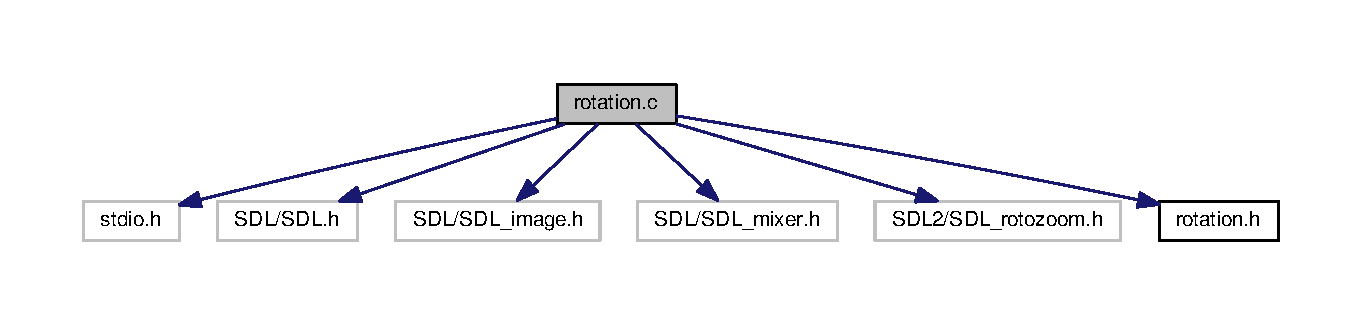
\includegraphics[width=350pt]{rotation_8c__incl}
\end{center}
\end{figure}
\subsection*{Functions}
\begin{DoxyCompactItemize}
\item 
void \hyperlink{rotation_8c_a97cb49d9583cdcb3814e7ae2c344c240}{rotationgauche} (S\+D\+L\+\_\+\+Event event, S\+D\+L\+\_\+\+Surface $\ast$image, S\+D\+L\+\_\+\+Surface $\ast$image2, S\+D\+L\+\_\+\+Surface $\ast$rotation, S\+D\+L\+\_\+\+Surface $\ast$screen, S\+D\+L\+\_\+\+Rect position1)
\begin{DoxyCompactList}\small\item\em fonction de la rotation a gauche \end{DoxyCompactList}\item 
void \hyperlink{rotation_8c_ab8622150bbd10e620d3b3afb1f4a7d3f}{rotationdroite} (S\+D\+L\+\_\+\+Event event, S\+D\+L\+\_\+\+Surface $\ast$image, S\+D\+L\+\_\+\+Surface $\ast$image2, S\+D\+L\+\_\+\+Surface $\ast$rotation, S\+D\+L\+\_\+\+Surface $\ast$screen, S\+D\+L\+\_\+\+Rect position1)
\begin{DoxyCompactList}\small\item\em fonction de la rotation a droite \end{DoxyCompactList}\end{DoxyCompactItemize}


\subsection{Function Documentation}
\index{rotation.\+c@{rotation.\+c}!rotationdroite@{rotationdroite}}
\index{rotationdroite@{rotationdroite}!rotation.\+c@{rotation.\+c}}
\subsubsection[{\texorpdfstring{rotationdroite(\+S\+D\+L\+\_\+\+Event event, S\+D\+L\+\_\+\+Surface $\ast$image, S\+D\+L\+\_\+\+Surface $\ast$image2, S\+D\+L\+\_\+\+Surface $\ast$rotation, S\+D\+L\+\_\+\+Surface $\ast$screen, S\+D\+L\+\_\+\+Rect position1)}{rotationdroite(SDL_Event event, SDL_Surface *image, SDL_Surface *image2, SDL_Surface *rotation, SDL_Surface *screen, SDL_Rect position1)}}]{\setlength{\rightskip}{0pt plus 5cm}void rotationdroite (
\begin{DoxyParamCaption}
\item[{S\+D\+L\+\_\+\+Event}]{event, }
\item[{S\+D\+L\+\_\+\+Surface $\ast$}]{image, }
\item[{S\+D\+L\+\_\+\+Surface $\ast$}]{image2, }
\item[{S\+D\+L\+\_\+\+Surface $\ast$}]{rotation, }
\item[{S\+D\+L\+\_\+\+Surface $\ast$}]{screen, }
\item[{S\+D\+L\+\_\+\+Rect}]{position1}
\end{DoxyParamCaption}
)}\hypertarget{rotation_8c_ab8622150bbd10e620d3b3afb1f4a7d3f}{}\label{rotation_8c_ab8622150bbd10e620d3b3afb1f4a7d3f}


fonction de la rotation a droite 


\begin{DoxyParams}{Parameters}
{\em evenement} & \\
\hline
{\em background} & \\
\hline
{\em image} & qui va subir la rotation \\
\hline
{\em rotation} & \\
\hline
{\em l\textquotesingle{}ecran} & \\
\hline
{\em position} & \\
\hline
\end{DoxyParams}
\index{rotation.\+c@{rotation.\+c}!rotationgauche@{rotationgauche}}
\index{rotationgauche@{rotationgauche}!rotation.\+c@{rotation.\+c}}
\subsubsection[{\texorpdfstring{rotationgauche(\+S\+D\+L\+\_\+\+Event event, S\+D\+L\+\_\+\+Surface $\ast$image, S\+D\+L\+\_\+\+Surface $\ast$image2, S\+D\+L\+\_\+\+Surface $\ast$rotation, S\+D\+L\+\_\+\+Surface $\ast$screen, S\+D\+L\+\_\+\+Rect position1)}{rotationgauche(SDL_Event event, SDL_Surface *image, SDL_Surface *image2, SDL_Surface *rotation, SDL_Surface *screen, SDL_Rect position1)}}]{\setlength{\rightskip}{0pt plus 5cm}void rotationgauche (
\begin{DoxyParamCaption}
\item[{S\+D\+L\+\_\+\+Event}]{event, }
\item[{S\+D\+L\+\_\+\+Surface $\ast$}]{image, }
\item[{S\+D\+L\+\_\+\+Surface $\ast$}]{image2, }
\item[{S\+D\+L\+\_\+\+Surface $\ast$}]{rotation, }
\item[{S\+D\+L\+\_\+\+Surface $\ast$}]{screen, }
\item[{S\+D\+L\+\_\+\+Rect}]{position1}
\end{DoxyParamCaption}
)}\hypertarget{rotation_8c_a97cb49d9583cdcb3814e7ae2c344c240}{}\label{rotation_8c_a97cb49d9583cdcb3814e7ae2c344c240}


fonction de la rotation a gauche 


\begin{DoxyParams}{Parameters}
{\em evenement} & \\
\hline
{\em background} & \\
\hline
{\em image} & qui va subir la rotation \\
\hline
{\em rotation} & \\
\hline
{\em l\textquotesingle{}ecran} & \\
\hline
{\em position} & \\
\hline
\end{DoxyParams}

\hypertarget{rotation_8h}{}\section{rotation.\+h File Reference}
\label{rotation_8h}\index{rotation.\+h@{rotation.\+h}}
This graph shows which files directly or indirectly include this file\+:
\nopagebreak
\begin{figure}[H]
\begin{center}
\leavevmode
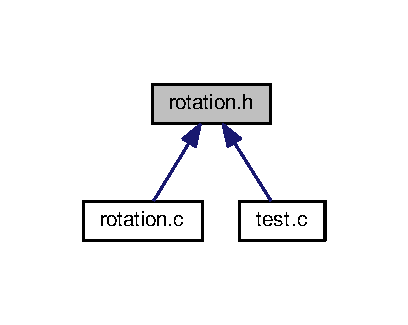
\includegraphics[width=196pt]{rotation_8h__dep__incl}
\end{center}
\end{figure}
\subsection*{Functions}
\begin{DoxyCompactItemize}
\item 
void \hyperlink{rotation_8h_a97cb49d9583cdcb3814e7ae2c344c240}{rotationgauche} (S\+D\+L\+\_\+\+Event event, S\+D\+L\+\_\+\+Surface $\ast$image, S\+D\+L\+\_\+\+Surface $\ast$image2, S\+D\+L\+\_\+\+Surface $\ast$rotation, S\+D\+L\+\_\+\+Surface $\ast$screen, S\+D\+L\+\_\+\+Rect position1)
\begin{DoxyCompactList}\small\item\em fonction de la rotation a gauche \end{DoxyCompactList}\item 
void \hyperlink{rotation_8h_ab8622150bbd10e620d3b3afb1f4a7d3f}{rotationdroite} (S\+D\+L\+\_\+\+Event event, S\+D\+L\+\_\+\+Surface $\ast$image, S\+D\+L\+\_\+\+Surface $\ast$image2, S\+D\+L\+\_\+\+Surface $\ast$rotation, S\+D\+L\+\_\+\+Surface $\ast$screen, S\+D\+L\+\_\+\+Rect position1)
\begin{DoxyCompactList}\small\item\em fonction de la rotation a droite \end{DoxyCompactList}\end{DoxyCompactItemize}


\subsection{Function Documentation}
\index{rotation.\+h@{rotation.\+h}!rotationdroite@{rotationdroite}}
\index{rotationdroite@{rotationdroite}!rotation.\+h@{rotation.\+h}}
\subsubsection[{\texorpdfstring{rotationdroite(\+S\+D\+L\+\_\+\+Event event, S\+D\+L\+\_\+\+Surface $\ast$image, S\+D\+L\+\_\+\+Surface $\ast$image2, S\+D\+L\+\_\+\+Surface $\ast$rotation, S\+D\+L\+\_\+\+Surface $\ast$screen, S\+D\+L\+\_\+\+Rect position1)}{rotationdroite(SDL_Event event, SDL_Surface *image, SDL_Surface *image2, SDL_Surface *rotation, SDL_Surface *screen, SDL_Rect position1)}}]{\setlength{\rightskip}{0pt plus 5cm}void rotationdroite (
\begin{DoxyParamCaption}
\item[{S\+D\+L\+\_\+\+Event}]{event, }
\item[{S\+D\+L\+\_\+\+Surface $\ast$}]{image, }
\item[{S\+D\+L\+\_\+\+Surface $\ast$}]{image2, }
\item[{S\+D\+L\+\_\+\+Surface $\ast$}]{rotation, }
\item[{S\+D\+L\+\_\+\+Surface $\ast$}]{screen, }
\item[{S\+D\+L\+\_\+\+Rect}]{position1}
\end{DoxyParamCaption}
)}\hypertarget{rotation_8h_ab8622150bbd10e620d3b3afb1f4a7d3f}{}\label{rotation_8h_ab8622150bbd10e620d3b3afb1f4a7d3f}


fonction de la rotation a droite 


\begin{DoxyParams}{Parameters}
{\em evenement} & \\
\hline
{\em background} & \\
\hline
{\em image} & qui va subir la rotation \\
\hline
{\em rotation} & \\
\hline
{\em l\textquotesingle{}ecran} & \\
\hline
{\em position} & \\
\hline
\end{DoxyParams}
\index{rotation.\+h@{rotation.\+h}!rotationgauche@{rotationgauche}}
\index{rotationgauche@{rotationgauche}!rotation.\+h@{rotation.\+h}}
\subsubsection[{\texorpdfstring{rotationgauche(\+S\+D\+L\+\_\+\+Event event, S\+D\+L\+\_\+\+Surface $\ast$image, S\+D\+L\+\_\+\+Surface $\ast$image2, S\+D\+L\+\_\+\+Surface $\ast$rotation, S\+D\+L\+\_\+\+Surface $\ast$screen, S\+D\+L\+\_\+\+Rect position1)}{rotationgauche(SDL_Event event, SDL_Surface *image, SDL_Surface *image2, SDL_Surface *rotation, SDL_Surface *screen, SDL_Rect position1)}}]{\setlength{\rightskip}{0pt plus 5cm}void rotationgauche (
\begin{DoxyParamCaption}
\item[{S\+D\+L\+\_\+\+Event}]{event, }
\item[{S\+D\+L\+\_\+\+Surface $\ast$}]{image, }
\item[{S\+D\+L\+\_\+\+Surface $\ast$}]{image2, }
\item[{S\+D\+L\+\_\+\+Surface $\ast$}]{rotation, }
\item[{S\+D\+L\+\_\+\+Surface $\ast$}]{screen, }
\item[{S\+D\+L\+\_\+\+Rect}]{position1}
\end{DoxyParamCaption}
)}\hypertarget{rotation_8h_a97cb49d9583cdcb3814e7ae2c344c240}{}\label{rotation_8h_a97cb49d9583cdcb3814e7ae2c344c240}


fonction de la rotation a gauche 


\begin{DoxyParams}{Parameters}
{\em evenement} & \\
\hline
{\em background} & \\
\hline
{\em image} & qui va subir la rotation \\
\hline
{\em rotation} & \\
\hline
{\em l\textquotesingle{}ecran} & \\
\hline
{\em position} & \\
\hline
\end{DoxyParams}

\hypertarget{SDL__rotozoom_8h}{}\section{S\+D\+L\+\_\+rotozoom.\+h File Reference}
\label{SDL__rotozoom_8h}\index{S\+D\+L\+\_\+rotozoom.\+h@{S\+D\+L\+\_\+rotozoom.\+h}}
{\ttfamily \#include $<$math.\+h$>$}\\*
{\ttfamily \#include \char`\"{}S\+D\+L.\+h\char`\"{}}\\*
Include dependency graph for S\+D\+L\+\_\+rotozoom.\+h\+:
\nopagebreak
\begin{figure}[H]
\begin{center}
\leavevmode
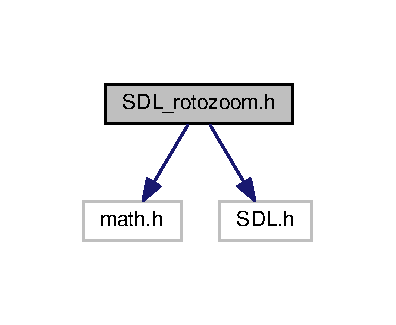
\includegraphics[width=190pt]{SDL__rotozoom_8h__incl}
\end{center}
\end{figure}
\subsection*{Classes}
\begin{DoxyCompactItemize}
\item 
struct \hyperlink{structtColorRGBA}{t\+Color\+R\+G\+BA}
\item 
struct \hyperlink{structtColorY}{t\+ColorY}
\end{DoxyCompactItemize}
\subsection*{Macros}
\begin{DoxyCompactItemize}
\item 
\#define {\bfseries M\+\_\+\+PI}~3.\+141592654\hypertarget{SDL__rotozoom_8h_ae71449b1cc6e6250b91f539153a7a0d3}{}\label{SDL__rotozoom_8h_ae71449b1cc6e6250b91f539153a7a0d3}

\item 
\#define {\bfseries S\+M\+O\+O\+T\+H\+I\+N\+G\+\_\+\+O\+FF}~0\hypertarget{SDL__rotozoom_8h_a6541cd06edcce77d8a6f1c6350c988af}{}\label{SDL__rotozoom_8h_a6541cd06edcce77d8a6f1c6350c988af}

\item 
\#define {\bfseries S\+M\+O\+O\+T\+H\+I\+N\+G\+\_\+\+ON}~1\hypertarget{SDL__rotozoom_8h_abeb6ae7618fcb315d0399fe65849a2e8}{}\label{SDL__rotozoom_8h_abeb6ae7618fcb315d0399fe65849a2e8}

\end{DoxyCompactItemize}
\subsection*{Typedefs}
\begin{DoxyCompactItemize}
\item 
typedef struct \hyperlink{structtColorRGBA}{t\+Color\+R\+G\+BA} {\bfseries t\+Color\+R\+G\+BA}\hypertarget{SDL__rotozoom_8h_a203fd84ecb148189f3afc137f6ce5141}{}\label{SDL__rotozoom_8h_a203fd84ecb148189f3afc137f6ce5141}

\item 
typedef struct \hyperlink{structtColorY}{t\+ColorY} {\bfseries t\+ColorY}\hypertarget{SDL__rotozoom_8h_a1bd6de894f36faa2d124c437462266eb}{}\label{SDL__rotozoom_8h_a1bd6de894f36faa2d124c437462266eb}

\end{DoxyCompactItemize}
\subsection*{Functions}
\begin{DoxyCompactItemize}
\item 
S\+D\+L\+\_\+\+Surface $\ast$ {\bfseries rotozoom\+Surface} (S\+D\+L\+\_\+\+Surface $\ast$src, double angle, double zoom, int smooth)\hypertarget{SDL__rotozoom_8h_a5f64ed53eeee5f2667971c857698d1e5}{}\label{SDL__rotozoom_8h_a5f64ed53eeee5f2667971c857698d1e5}

\item 
S\+D\+L\+\_\+\+Surface $\ast$ {\bfseries zoom\+Surface} (S\+D\+L\+\_\+\+Surface $\ast$src, double zoomx, double zoomy, int smooth)\hypertarget{SDL__rotozoom_8h_abdd772b2f6b1f26134e4e90cda657a21}{}\label{SDL__rotozoom_8h_abdd772b2f6b1f26134e4e90cda657a21}

\end{DoxyCompactItemize}


\subsection{Detailed Description}
Bibliotheque S\+DL necessaire pour la rotation et le zoom 
\hypertarget{test_8c}{}\section{test.\+c File Reference}
\label{test_8c}\index{test.\+c@{test.\+c}}


pour tester la rotation automatique  


{\ttfamily \#include $<$stdio.\+h$>$}\\*
{\ttfamily \#include \char`\"{}S\+D\+L/\+S\+D\+L.\+h\char`\"{}}\\*
{\ttfamily \#include \char`\"{}S\+D\+L/\+S\+D\+L\+\_\+image.\+h\char`\"{}}\\*
{\ttfamily \#include \char`\"{}S\+D\+L/\+S\+D\+L\+\_\+mixer.\+h\char`\"{}}\\*
{\ttfamily \#include \char`\"{}S\+D\+L2/\+S\+D\+L\+\_\+rotozoom.\+h\char`\"{}}\\*
{\ttfamily \#include \char`\"{}rotation.\+h\char`\"{}}\\*
Include dependency graph for test.\+c\+:
\nopagebreak
\begin{figure}[H]
\begin{center}
\leavevmode
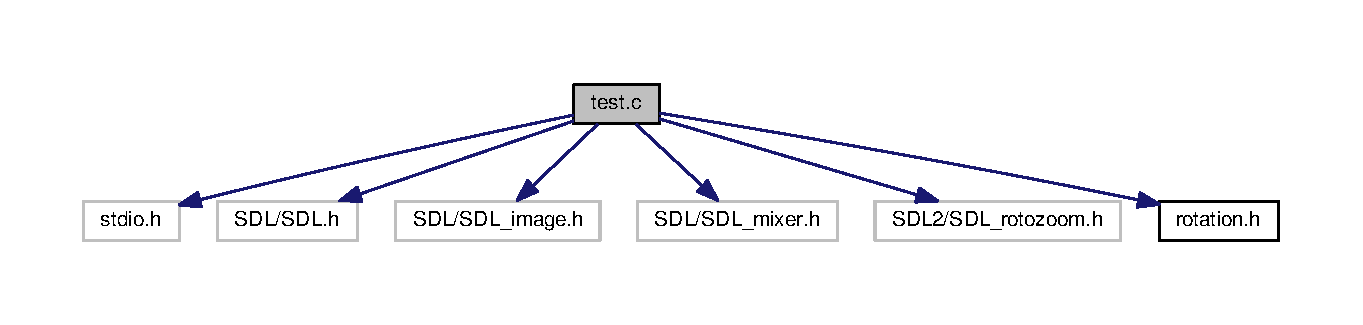
\includegraphics[width=350pt]{test_8c__incl}
\end{center}
\end{figure}
\subsection*{Functions}
\begin{DoxyCompactItemize}
\item 
int {\bfseries main} (void)\hypertarget{test_8c_a840291bc02cba5474a4cb46a9b9566fe}{}\label{test_8c_a840291bc02cba5474a4cb46a9b9566fe}

\end{DoxyCompactItemize}


\subsection{Detailed Description}
pour tester la rotation automatique 

\begin{DoxyAuthor}{Author}
Ramy Klouz 
\end{DoxyAuthor}

%--- End generated contents ---

% Index
\backmatter
\newpage
\phantomsection
\clearemptydoublepage
\addcontentsline{toc}{chapter}{Index}
\printindex

\end{document}
